\documentclass[amsmath,amssymb,notitlepage,12pt]{revtex4-1}
\usepackage{graphicx}
\usepackage{bm}% bold math
\usepackage{multirow}
\usepackage{booktabs}
\usepackage{verbatim}
\usepackage{hyperref}
\hypersetup{pdftex,colorlinks=true,allcolors=blue}
\usepackage{hypcap}
%\usepackage[small,compact]{titlesec}
%\usepackage{showkeys}
%\addtolength{\textheight}{0.3cm}
%\addtolength{\topmargin}{-0.15cm}
%\addtolength{\textwidth}{0.4cm}
%\addtolength{\hoffset}{-0.2cm}
\begin{document}
\hspace*{11.5cm}\texttt{HPS-NOTE 2015-XXX}

\title{ECal Pulse Fitting}
\author{N. Baltzell}
\affiliation{Jefferson Lab}
\date{\today}
\begin{abstract}
In the HPS 2015 Engineering Run we readout and recorded the full waveform in 4 ns samples from the calorimeter's FADC250 modules. 
To extract pulse energy and time, Minuit fitting was implemented in the offline \texttt{hps-java} framework.
Here we first describe the methods previously used to reconstruct HPS ECal pulses from waveforms, and then describe the new fitting method and its improvements on energy and time resolution.
\end{abstract}
\maketitle

\section{FADC250 Modes}
The FADC250 module samples at 250 MHz, or once every 4 ns, and its firmware can be configured to readout in various modes, all of which are some combination of:
\begin{itemize}
  \item Mode-1:  Full waveform.
  \item Mode-3:  Sample \# of threshold crossing and arithmetic pulse integral.  
  \item Mode-7:  {\em High-resolution} time and arithmetic pulse integral, and a pedestal and pulse maximum.
\end{itemize}
The decision to readout a given channel is the same for all modes and based only on a leading edge threshold.
In the 2014 Commissioning Run we recorded data in all three of the above modes for testing, while in the Spring 2015 Engineering Run we used only Mode-1.  In all cases we used a readout threshold of FADC=12.
We can also apply the firmware's Mode-3 and Mode-7 algorithms offline to reconstruct pulses from data readout in Mode-1.

\subsection{Pulse Time}
Mode-3's pulse time is calculated using the same algorithm the trigger uses for hit and cluster coincidence requirements and is just the time of leading-edge threshold crossing with 4 ns resolution.  We mainly apply the Mode-3 timing algorithm offline only to emulate the trigger for diagnostics.  Mode-3 timing requires the largest time-walk correction in offline reconstruction and results in the worst resolution of the options studied.

The Mode-7 timing algorithm is more sophisticated and starts by calculating a pedestal from the first 4 samples at the beginning of the window. Next it finds the pulse maximum after threshold crossing.  Then the two samples before and after half-height crossing are linearly interpolated to calculate the pulse time at half-height (see Figure~\ref{fig:mode7}).  This gives a significantly better resolution than Mode-3 and is much less affected by time-walk (see Figure~\ref{fig:timeWalk}).
\begin{figure}[htbp]\centering\hspace{-2cm}
  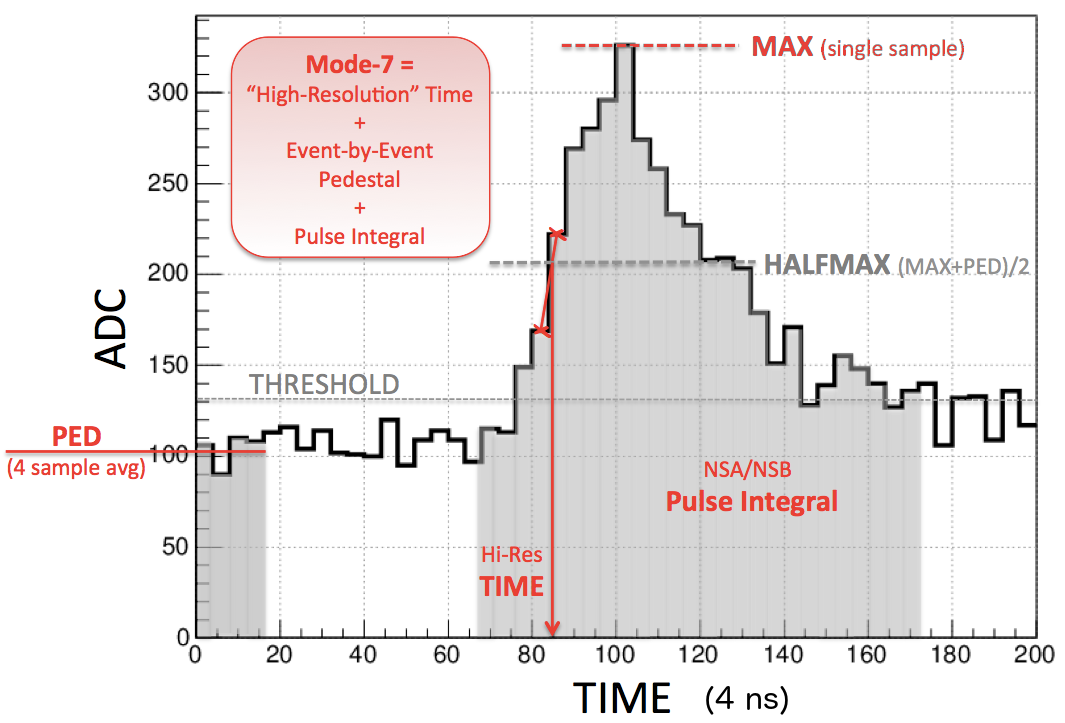
\includegraphics[width=14cm]{pics/mode7.png}
  \caption{An illustration of Mode-1 readout (full waveform) and Mode-7 readout (in red).\label{fig:mode7}}
\end{figure}

\subsection{Pulse Integral}
Mode-3 and Mode-7 pulse integrals simply sum the discrete FADC distribution over a fixed range relative to threshold crossing.  The number of samples integrated over before and after threshold crossing has so far always beens set to 5 and 25 (20 and 100 ns) for HPS's calorimeter.  The integral is truncated at the edges of the readout window, which was set to 200 ns with our trigger pulses centered near $^\sim$50 ns. No pedestal is subtracted in the readout in any mode and must be accounted for offline, although the trigger does use an online pedestal subtraction for its decisions.  
\begin{figure}[htbp]\centering
  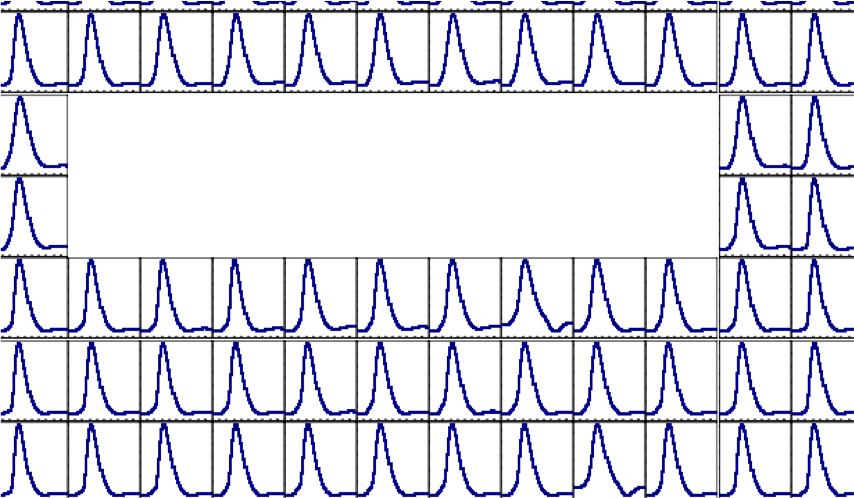
\includegraphics[width=12cm,trim={0 0 0 0.2cm},clip]{pics/avgpulses.png}
  \caption{Pulses averaged over many events for example channels near the beamline.\label{fig:avgPulses}}
\end{figure}

\section{Pulse Fitting}
For data recorded in Mode-1, full waveform, we considered an additional method for extracting pulse information that may allow more precise measures of time and
energy, as well as reduction of pileup effects in energy measurements.  
The calorimeter's FADC response is expected to be well described by the sum of a pedestal $P$ and a {\em 3-pole} function for the pulse with width $\tau$ and pulse time $t_0$~\cite{hpsnote2014002}:
\begin{equation}
  P\ +\ \frac{A}{2\tau^3}\ (t-t_0)^2\ e^{-(t-t_0)/\tau}
  \label{eqn:3pole}
\end{equation}
where for $t<t_0$ the pulse amplitude is implicitly zero.  This function is normalized such that $A$ is the pulse integral.  The $\tau$ parameter is also half of the rise time, the duration between pedestal and pulse maximum.

This {\em 3-pole} function is used to fit each waveform via the AIDA interface to Minuit in \texttt{hps-java}.  If the fit fails to converge, reconstruction falls back to the Mode-7 algorithm for energy and time.

\subsection{Parameter Initialization}
Initialization of fit parameters is based on the data, independently for every event and channel. 
The pedestal parameter is initialized from samples before threshold crossing.
The pulse integral is initialized as the pedestal-subtracted arithmetic FADC sum.
And the pulse time is initialized according to the value determined from ``Mode-7'' high-resolution timing with a fixed offset to account for pulse rise time.

\subsection{Pulse Width}
In initial attempts, the pulse width $\tau$ was allowed to be a free fit parameter.  However, the pulse shape from the calorimeter is dominated by the preamplifiers and should be very constant and independent of energy.
We do see what may be a small energy-dependence, but it is much smaller than the channel to channel variations in pulse width (see Figure~\ref{fig:pulseWidths}).

Pulses from all 442 channels were fit with the {\em 3-pole} function while letting the width be a free parameter.
The resulting average width for each channel was uploaded to the conditions database (table \texttt{ecal\_pulse\_widths}) and used to fix the width parameter for each channel independently.  Fixing the widths in pulse fitting did significantly improve timing resolution relative to free widths.

\subsection{Pedestal}
Studies were done regarding whether the pedestal should be a free parameter in the fit.  The conclusion was unclear as to whether free or fixed width was superior, as neither resulted in a significantly better result in terms of energy nor time resolution, nor aesthetically better fits.  For what is shown here, and currently the default in \texttt{hps-java}, the pedestal is a free parameter, although fixing it can be enabled with a flag in the steering file.

\subsection{Fit Range}
In order to include the data's pedestal in the fit, and allow the fit to account for fluctuations in the pedestal, the fit range was set to start 20 ns before threshold crossing. 
And while the full calorimeter pulse lasts for $^\sim$100 ns, the fit range is currently truncated at 60 ns past threshold crossing.
This allows to be less sensitive to pileup pulses and deviations from the {\em 3-pole} form in the pulse tail as will be shown in the next section. 

\subsection{Optimization}
Using Minuit to fit ECal pulses in \texttt{hps-java} increases CPU time for conversion of raw FADC waveform to energy/time by factor of $^\sim$5 relative to the previous algorithms.
This is still only 10\% of total HPS reconstruction time and not currently a problem, but some steps to economize were taken. 

For one, fitting is only attempted for pulses around the trigger time, while for pulses far from the trigger time the Mode-7 algorithms are used.  Achieveing reliable fit results is also more difficult for pulses near the edge of the window.

Also, limits are placed on the pulse time fit parameter to be well within the readout window.  Otherwise, Minuit will iterate needlessly when the parameter surpasses the window's edge due to insensitivy to the data.

If more speed is necessary in the future, we will most likely need to implement some dedicated fitting algorithm instead of using the general purpose Minuit.
\begin{figure}[htbp]\centering
  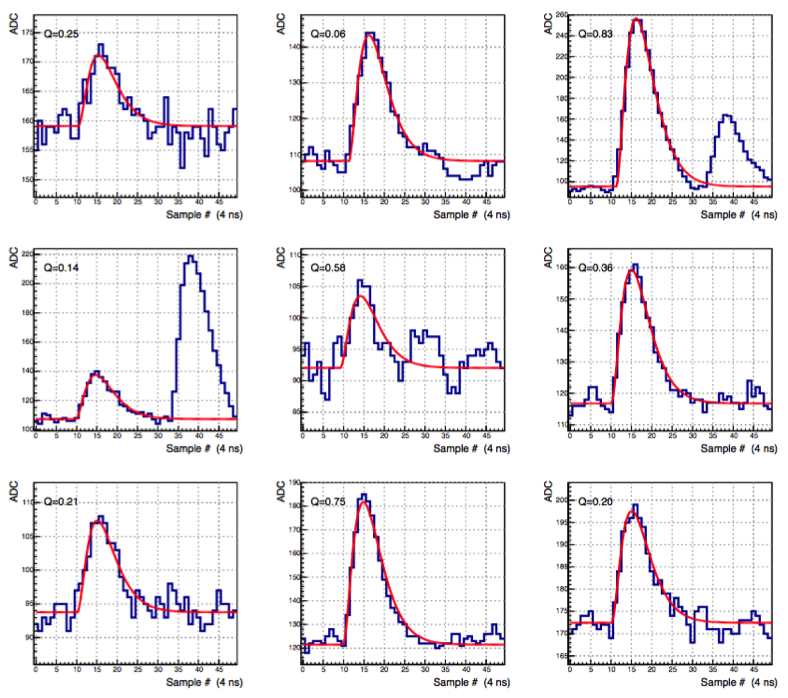
\includegraphics[width=13cm]{pics/pulseFits.png}
  \caption{Example fits of individual pulses.  The resulting {\em 3-pole} function is drawn across the entire readout window for visualization, although the actual range fitted is smaller (see text).\label{fig:pulseFits}}
\end{figure}

\section{Results}
\subsection{Fit Quality}
The quality of the fits can first be assessed by eye.  Figure~\ref{fig:pulseFits} shows an unbiased sample of fits from various channels, unbiased in the sense that it is one fit for every readout with no selection.  Many more additional fits with the same lack of criteria are available online~\cite{miscfits}.

One observation is that the fit method does a reasonable job of ignoring pileup pulses.  This is due largely to restricting the fit range to 60 ns after threshold crossing.
Another is that this {\em 3-pole} function does not describe the tail of our real ECal pulse.  Around 90 ns after threshold crossing there is a reflection below pedestal in all channels, evident in Figure~\ref{fig:avgPulses} but also visible in the single pulse fits in Figure~\ref{fig:pulseFits}.

The $\chi^2$ distribution of the fits is shown in Figure~\ref{fig:chi2}.  While it does have the expected shape, it is clearly peaked far too low.  It was found the FADC noise, used as uncertainties in the fitting, were overestimated by a factor of $\sqrt{2}$.  After correcting for this the peak sits at about $\chi^2$=0.7.  However, this has zero effect on the resulting fit parameter results since all FADC samples are assumed to have the same noise level for a given channel.
\begin{figure}[htbp]\centering
  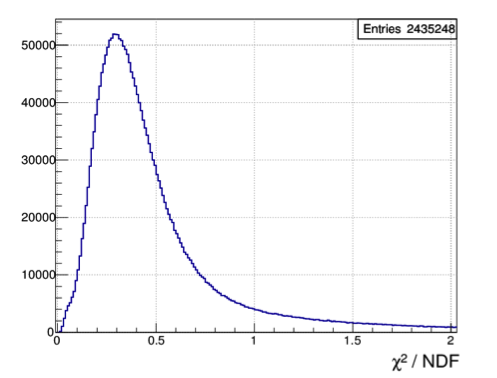
\includegraphics[width=8cm]{pics/chi2.png}
  \caption{$\chi^2$ distribution from the {\em 3-pole} fits.  The noise level was overestimated (see text).\label{fig:chi2}}
\end{figure}

\subsection{Timing}
The pulse time from {\em 3-pole} fitting is taken as the $t_0$ in Equation~\ref{eqn:3pole}.  With pulse widths left as a free fit parameter, the time resolution was clearly worse than the Mode-7 timing algorithm.  After fixing each channel's pulse width to its average, the resolution became slightly better than Mode-7 (see Figure~\ref{fig:timeReso}).  
The plots shown here are before accounting for channel timing skews, after which a high energy timing resolution below 400 ns is achieved~\cite{timingCalibration}.

  The time-walk from pulse fitting is also sgnificantly less than Mode-7 timing algorithms (see Figure~\ref{fig:timeWalk}), which can be attributed to a better description of pulse shape.
\begin{figure}[htbp]\centering
  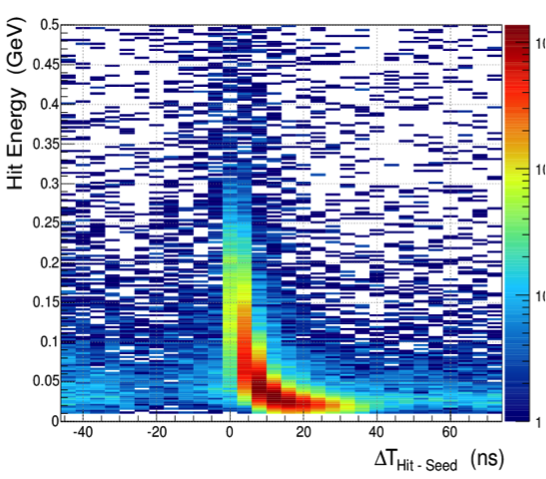
\includegraphics[width=5.2cm,height=5cm]{pics/mode3tw.png}
  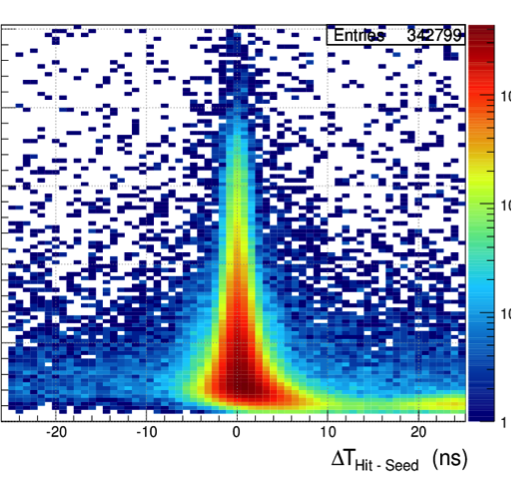
\includegraphics[width=5cm,height=5cm]{pics/mode7tw.png}
  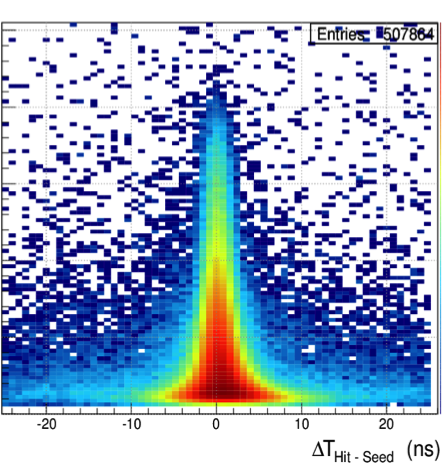
\includegraphics[width=5cm,height=5cm]{pics/fittw.png}
  \caption{Hit energy versus difference between seed and hit times for three different methods of extracting pulse times:  Mode-3 (left), Mode-7 (center), and {\em 3-pole} fitting (right).  Note the time axis scale for Mode-3 is three times larger than the others.\label{fig:timeWalk}}
\end{figure}
\begin{figure}[htbp]\centering
  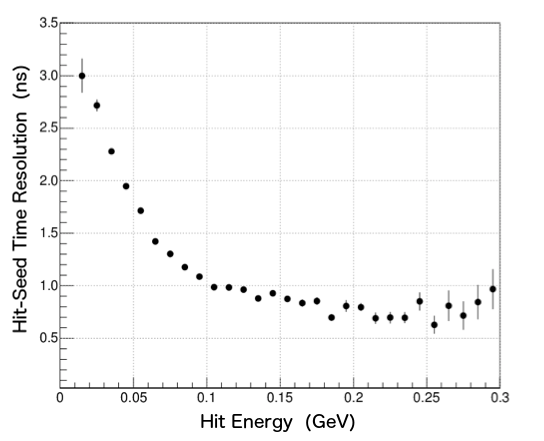
\includegraphics[height=6.1cm,width=7cm]{pics/mode7reso.png}
  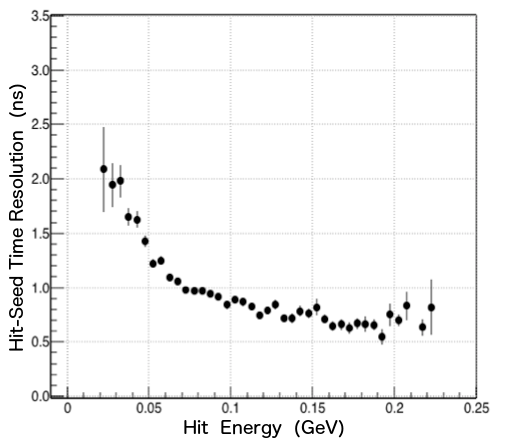
\includegraphics[width=7cm]{pics/fitreso.png}
  \caption{Time resolution as function of hit energy for Mode-7 (left) and {\em 3-pole} fitting (right).  This is based on comparing hit and seed time and is before calibration for crystal time offsets.\label{fig:timeReso}}
\end{figure}
\begin{figure}[htbp]\centering
  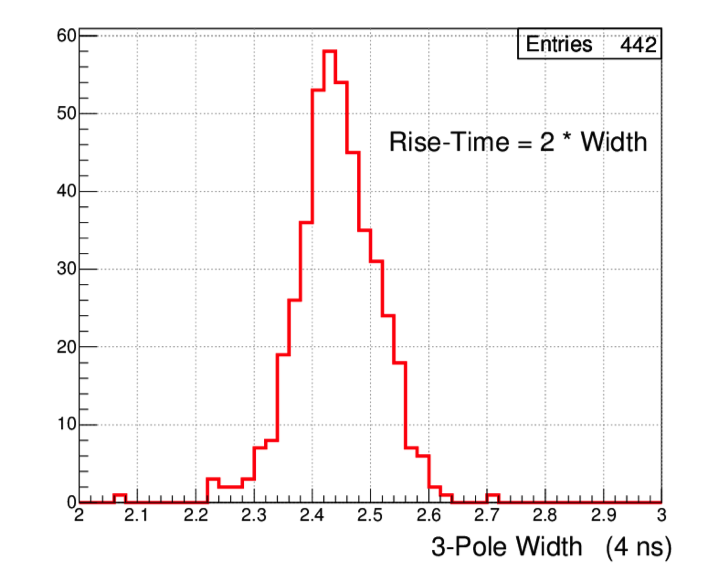
\includegraphics[height=6cm]{pics/pulseWidths.png}
  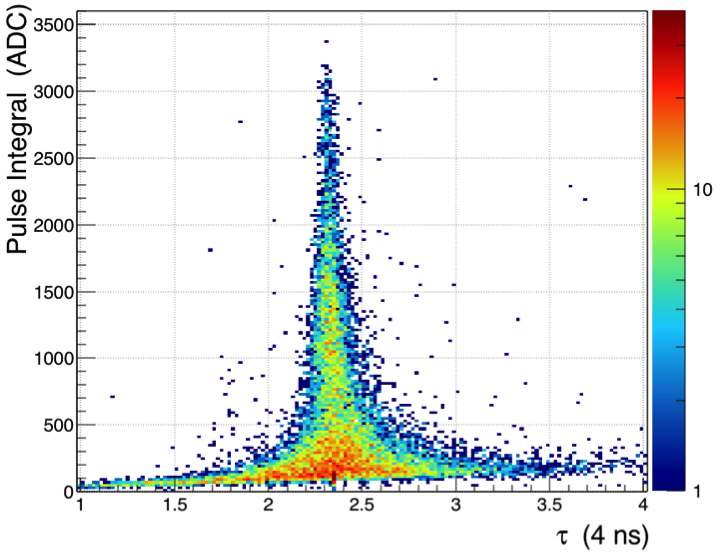
\includegraphics[height=5.9cm]{pics/pulseWidthEnergy.png}
  \caption{Distribution of average fitted pulse widths for the 442 ECal channels (left).  Energy dependence of fitted pulse widths for one channel (right).\label{fig:pulseWidths}}
\end{figure}

\subsection{Energy}
Significant improvement in ECal energy resolution is found due to pulse fitting relative to arithmetic FADC pulse integrals (see Table~\ref{tab:reso}).  This is evident in single-cluster energy in Figure~\ref{fig:fee}, measured via elastic scattering off Tungsten where the measured electron carries basically the full beam energy of 1.05 GeV.  It is also clear in the two-cluster energy sum in Figure~\ref{fig:moller}, measured via M\o ller scattering where the measured electrons share the beam energy.
\begin{table}[htbp]\centering
  \begin{tabular}{lccc|ccc}\cmidrule[1.5pt]{1-7}
    & \multicolumn{3}{c}{Elastic} & \multicolumn{3}{|c}{M\o ller} \\\cmidrule[1pt]{2-7}
    & $\mu$ & $\sigma$ & $\sigma/\mu$ & $\mu$ & $\sigma$ & $\sigma/\mu$ \\\cmidrule[1.5pt]{1-7}
    \multicolumn{1}{l}{ADC Sum} &\ \ 818\ &\ 63\ &\ 7.6\%\ \ &\ \ 787\ &\ 54\ &\ 6.8\%\ \ \\
    \multicolumn{1}{l}{Fitting} &\ \ 877\ &\ 58\ &\ 6.6\%\ \ &\ \ 843\ &\ 49\ &\ 5.8\%\ \ \\
    \bottomrule[1.5pt]
  \end{tabular}
  \caption{Cluster energy peak positions and resolutions in MeV for the ADC summing method and the new pulse fitting method.  Note these are both before final gain and timing calibration.\label{tab:reso}}
\end{table}

Based on simulation, the expected measured cluster energy for elastics with a beam energy of 1.05 GeV is $^\sim$0.89 GeV, while for M\o llers the expected energy sum is slightly less due to the lower energy electrons and larger fractional shower loss.  Note these plots are using channel gains derived from cosmics, with only 18 MeV energy deposition, before our final gain calibrations based on higher energy clusters.

It is worthwhile to note that both elastic and M\o ller energy peak positions increase while their widths simultaneously decrease.  If the width instead scaled with energy, it could be attributed to just a mathematical scaling effect.

Further confirmation of the improvement is evident in energy resolutions binned by seed crystal in Figure~\ref{fig:feeReso}.  Almost all channels improve in energy resolution and none worsen.
\begin{figure}[htbp]\centering
  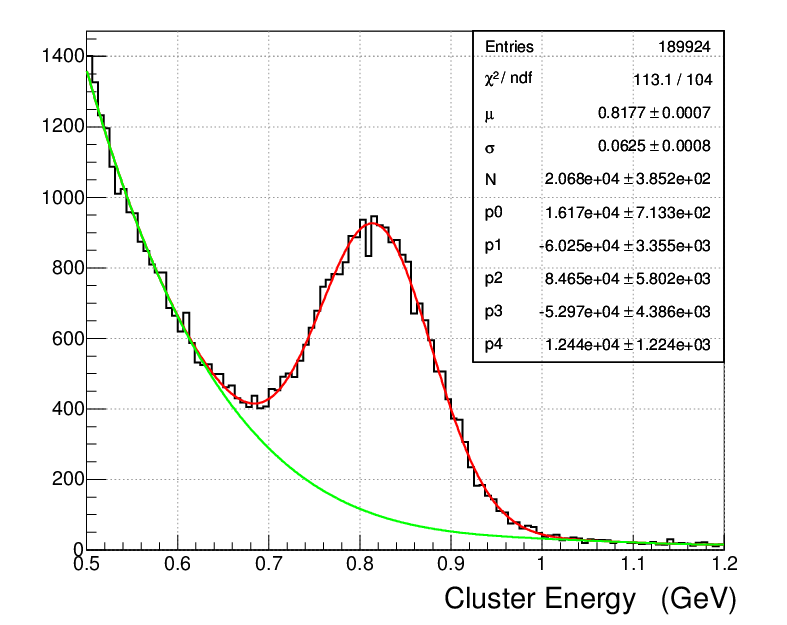
\includegraphics[width=8cm]{pics/fee.png}
  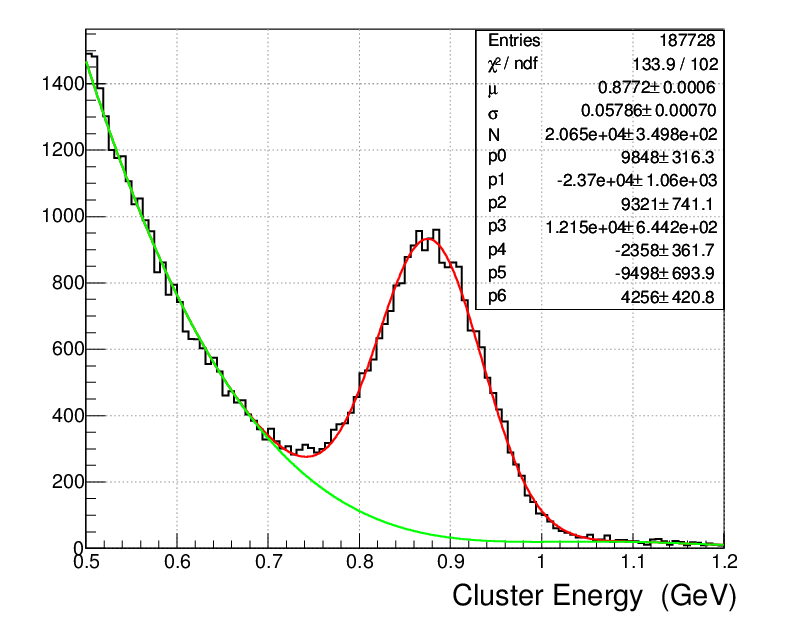
\includegraphics[width=8cm]{pics/fee3pole.png}
  \caption{Elastically scattered electron energy before (left) and after (right) pulse fitting.\label{fig:fee}}
\end{figure}
\begin{figure}[htbp]\centering
  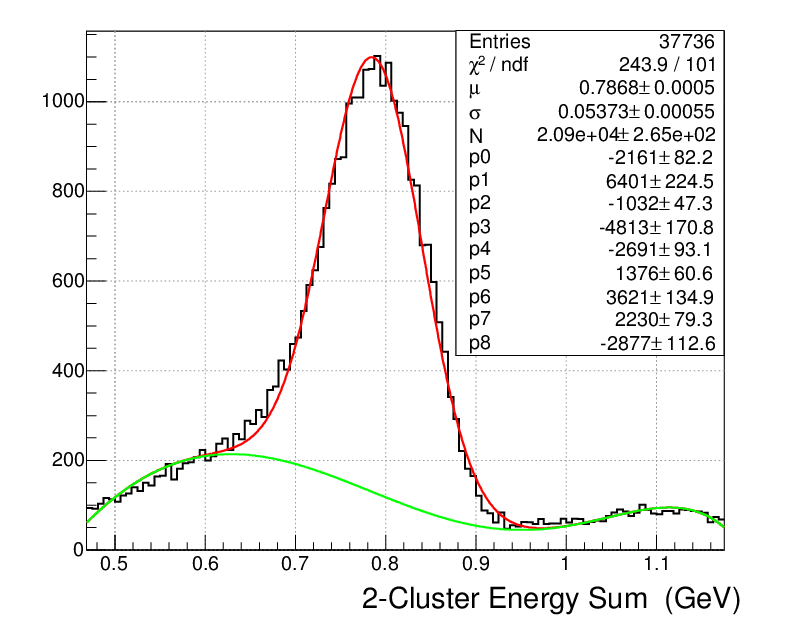
\includegraphics[width=8cm]{pics/moller.png}
  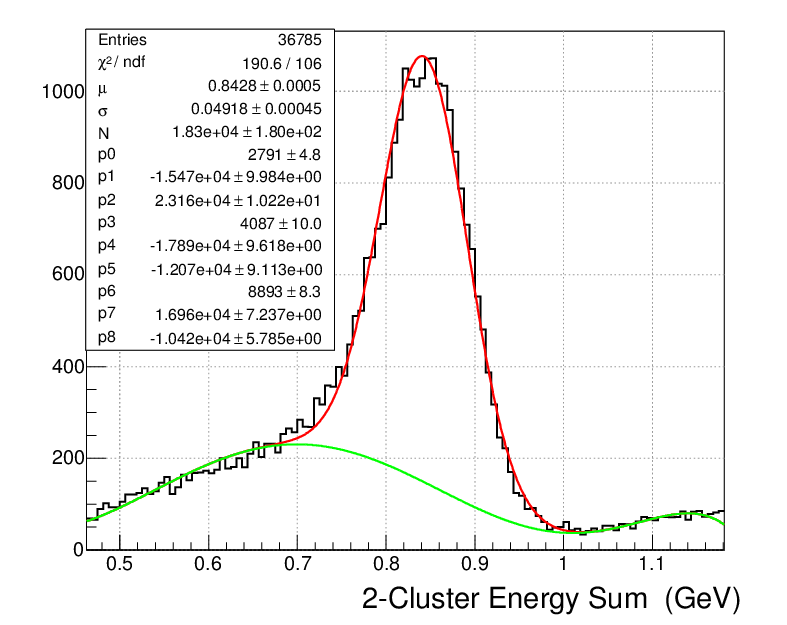
\includegraphics[width=8cm]{pics/moller3pole.png}
  \caption{M\o ller scattered $e^-e^-$ energy sum before (left) and after (right) pulse fitting.\label{fig:moller}}
\end{figure}
\begin{figure}[htbp]\centering
  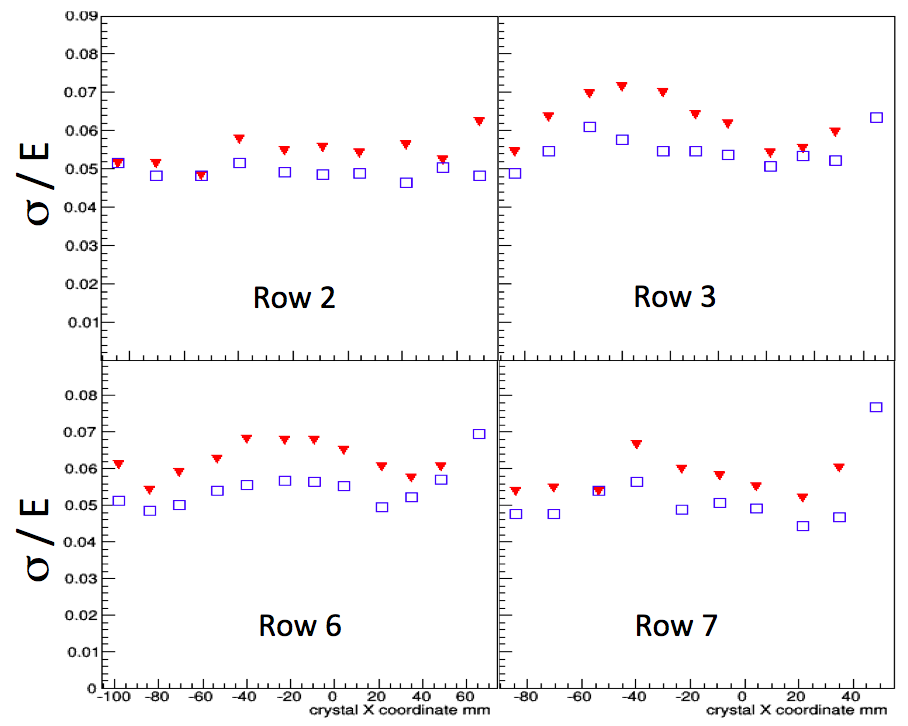
\includegraphics[width=12cm]{pics/feeReso.png}
  \caption{Energy resolution measured from elastic scattering, binned by seed crystal for channels near the beamline, before (red) and after (blue) pulse fitting.  Plot from R. Paremuzyan.\label{fig:feeReso}}
\end{figure}

\section{Conclusion}
Improvement in both energy and time resolution is achieved by fitting ECal waveforms with a {\em 3-pole} function instead of the previously used methods we adopted from the FADC250 firmware algorithms.  The fitting methods are implemented in \texttt{hps-java}'s reconstruction code in the package \texttt{org.hps.recon.ecal} and its classes \texttt{EcalPulseFitter} and \texttt{Ecal3PoleFunction} and were first used for the 2015 Engineering Run's {\em pass-1}. 

\bibliography{pulsefit}
\end{document}

